\documentclass[1p]{elsarticle_modified}
%\bibliographystyle{elsarticle-num}

%\usepackage[colorlinks]{hyperref}
%\usepackage{abbrmath_seonhwa} %\Abb, \Ascr, \Acal ,\Abf, \Afrak
\usepackage{amsfonts}
\usepackage{amssymb}
\usepackage{amsmath}
\usepackage{amsthm}
\usepackage{scalefnt}
\usepackage{amsbsy}
\usepackage{kotex}
\usepackage{caption}
\usepackage{subfig}
\usepackage{color}
\usepackage{graphicx}
\usepackage{xcolor} %% white, black, red, green, blue, cyan, magenta, yellow
\usepackage{float}
\usepackage{setspace}
\usepackage{hyperref}

\usepackage{tikz}
\usetikzlibrary{arrows}

\usepackage{multirow}
\usepackage{array} % fixed length table
\usepackage{hhline}

%%%%%%%%%%%%%%%%%%%%%
\makeatletter
\renewcommand*\env@matrix[1][\arraystretch]{%
	\edef\arraystretch{#1}%
	\hskip -\arraycolsep
	\let\@ifnextchar\new@ifnextchar
	\array{*\c@MaxMatrixCols c}}
\makeatother %https://tex.stackexchange.com/questions/14071/how-can-i-increase-the-line-spacing-in-a-matrix
%%%%%%%%%%%%%%%

\usepackage[normalem]{ulem}

\newcommand{\msout}[1]{\ifmmode\text{\sout{\ensuremath{#1}}}\else\sout{#1}\fi}
%SOURCE: \msout is \stkout macro in https://tex.stackexchange.com/questions/20609/strikeout-in-math-mode

\newcommand{\cancel}[1]{
	\ifmmode
	{\color{red}\msout{#1}}
	\else
	{\color{red}\sout{#1}}
	\fi
}

\newcommand{\add}[1]{
	{\color{blue}\uwave{#1}}
}

\newcommand{\replace}[2]{
	\ifmmode
	{\color{red}\msout{#1}}{\color{blue}\uwave{#2}}
	\else
	{\color{red}\sout{#1}}{\color{blue}\uwave{#2}}
	\fi
}

\newcommand{\Sol}{\mathcal{S}} %segment
\newcommand{\D}{D} %diagram
\newcommand{\A}{\mathcal{A}} %arc


%%%%%%%%%%%%%%%%%%%%%%%%%%%%%5 test

\def\sl{\operatorname{\textup{SL}}(2,\Cbb)}
\def\psl{\operatorname{\textup{PSL}}(2,\Cbb)}
\def\quan{\mkern 1mu \triangleright \mkern 1mu}

\theoremstyle{definition}
\newtheorem{thm}{Theorem}[section]
\newtheorem{prop}[thm]{Proposition}
\newtheorem{lem}[thm]{Lemma}
\newtheorem{ques}[thm]{Question}
\newtheorem{cor}[thm]{Corollary}
\newtheorem{defn}[thm]{Definition}
\newtheorem{exam}[thm]{Example}
\newtheorem{rmk}[thm]{Remark}
\newtheorem{alg}[thm]{Algorithm}

\newcommand{\I}{\sqrt{-1}}
\begin{document}

%\begin{frontmatter}
%
%\title{Boundary parabolic representations of knots up to 8 crossings}
%
%%% Group authors per affiliation:
%\author{Yunhi Cho} 
%\address{Department of Mathematics, University of Seoul, Seoul, Korea}
%\ead{yhcho@uos.ac.kr}
%
%
%\author{Seonhwa Kim} %\fnref{s_kim}}
%\address{Center for Geometry and Physics, Institute for Basic Science, Pohang, 37673, Korea}
%\ead{ryeona17@ibs.re.kr}
%
%\author{Hyuk Kim}
%\address{Department of Mathematical Sciences, Seoul National University, Seoul 08826, Korea}
%\ead{hyukkim@snu.ac.kr}
%
%\author{Seokbeom Yoon}
%\address{Department of Mathematical Sciences, Seoul National University, Seoul, 08826,  Korea}
%\ead{sbyoon15@snu.ac.kr}
%
%\begin{abstract}
%We find all boundary parabolic representation of knots up to 8 crossings.
%
%\end{abstract}
%\begin{keyword}
%    \MSC[2010] 57M25 
%\end{keyword}
%
%\end{frontmatter}

%\linenumbers
%\tableofcontents
%
\newcommand\colored[1]{\textcolor{white}{\rule[-0.35ex]{0.8em}{1.4ex}}\kern-0.8em\color{red} #1}%
%\newcommand\colored[1]{\textcolor{white}{ #1}\kern-2.17ex	\textcolor{white}{ #1}\kern-1.81ex	\textcolor{white}{ #1}\kern-2.15ex\color{red}#1	}

{\Large $\underline{12n_{0548}~(K12n_{0548})}$}

\setlength{\tabcolsep}{10pt}
\renewcommand{\arraystretch}{1.6}
\vspace{1cm}\begin{tabular}{m{100pt}>{\centering\arraybackslash}m{274pt}}
\multirow{5}{120pt}{
	\centering
	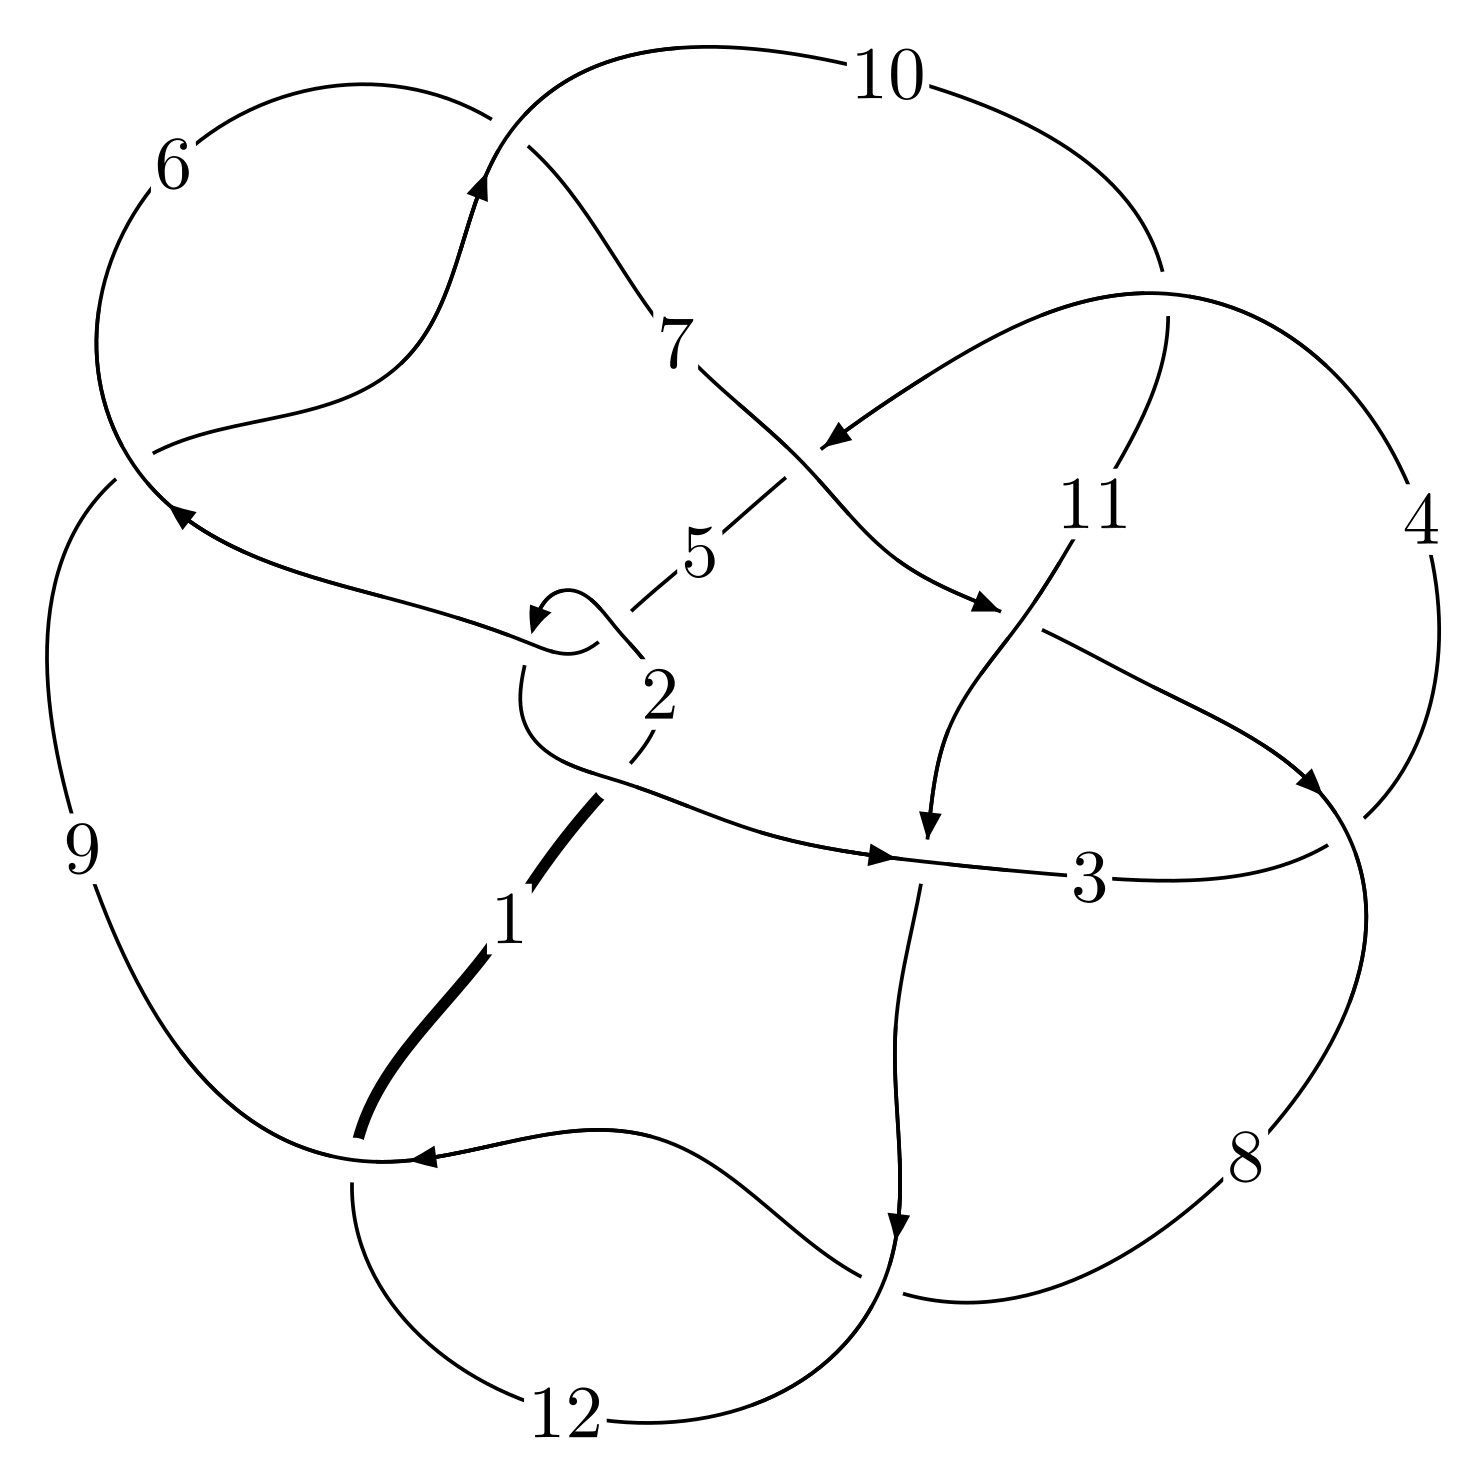
\includegraphics[width=112pt]{../../../GIT/diagram.site/Diagrams/png/2637_12n_0548.png}\\
\ \ \ A knot diagram\footnotemark}&
\allowdisplaybreaks
\textbf{Linearized knot diagam} \\
\cline{2-2}
 &
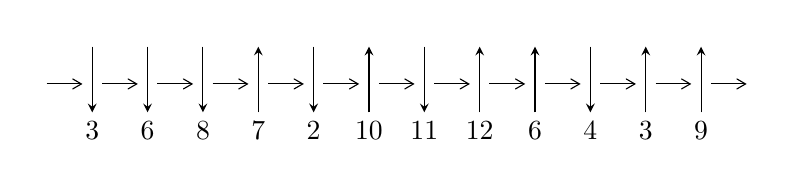
\begin{tikzpicture}[x=20pt, y=17pt]
	% nodes
	\node (C0) at (0, 0) {};
	\node (C1) at (1, 0) {};
	\node (C1U) at (1, +1) {};
	\node (C1D) at (1, -1) {3};

	\node (C2) at (2, 0) {};
	\node (C2U) at (2, +1) {};
	\node (C2D) at (2, -1) {6};

	\node (C3) at (3, 0) {};
	\node (C3U) at (3, +1) {};
	\node (C3D) at (3, -1) {8};

	\node (C4) at (4, 0) {};
	\node (C4U) at (4, +1) {};
	\node (C4D) at (4, -1) {7};

	\node (C5) at (5, 0) {};
	\node (C5U) at (5, +1) {};
	\node (C5D) at (5, -1) {2};

	\node (C6) at (6, 0) {};
	\node (C6U) at (6, +1) {};
	\node (C6D) at (6, -1) {10};

	\node (C7) at (7, 0) {};
	\node (C7U) at (7, +1) {};
	\node (C7D) at (7, -1) {11};

	\node (C8) at (8, 0) {};
	\node (C8U) at (8, +1) {};
	\node (C8D) at (8, -1) {12};

	\node (C9) at (9, 0) {};
	\node (C9U) at (9, +1) {};
	\node (C9D) at (9, -1) {6};

	\node (C10) at (10, 0) {};
	\node (C10U) at (10, +1) {};
	\node (C10D) at (10, -1) {4};

	\node (C11) at (11, 0) {};
	\node (C11U) at (11, +1) {};
	\node (C11D) at (11, -1) {3};

	\node (C12) at (12, 0) {};
	\node (C12U) at (12, +1) {};
	\node (C12D) at (12, -1) {9};
	\node (C13) at (13, 0) {};

	% arrows
	\draw[->,>={angle 60}]
	(C0) edge (C1) (C1) edge (C2) (C2) edge (C3) (C3) edge (C4) (C4) edge (C5) (C5) edge (C6) (C6) edge (C7) (C7) edge (C8) (C8) edge (C9) (C9) edge (C10) (C10) edge (C11) (C11) edge (C12) (C12) edge (C13) ;	\draw[->,>=stealth]
	(C1U) edge (C1D) (C2U) edge (C2D) (C3U) edge (C3D) (C4D) edge (C4U) (C5U) edge (C5D) (C6D) edge (C6U) (C7U) edge (C7D) (C8D) edge (C8U) (C9D) edge (C9U) (C10U) edge (C10D) (C11D) edge (C11U) (C12D) edge (C12U) ;
	\end{tikzpicture} \\
\hhline{~~} \\& 
\textbf{Solving Sequence} \\ \cline{2-2} 
 &
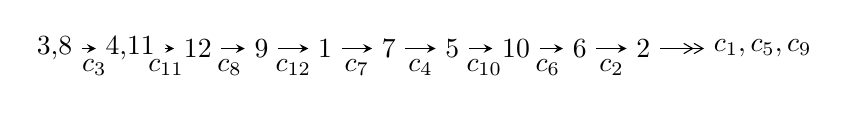
\begin{tikzpicture}[x=23pt, y=7pt]
	% node
	\node (A0) at (-1/8, 0) {3,8};
	\node (A1) at (17/16, 0) {4,11};
	\node (A2) at (17/8, 0) {12};
	\node (A3) at (25/8, 0) {9};
	\node (A4) at (33/8, 0) {1};
	\node (A5) at (41/8, 0) {7};
	\node (A6) at (49/8, 0) {5};
	\node (A7) at (57/8, 0) {10};
	\node (A8) at (65/8, 0) {6};
	\node (A9) at (73/8, 0) {2};
	\node (C1) at (1/2, -1) {$c_{3}$};
	\node (C2) at (13/8, -1) {$c_{11}$};
	\node (C3) at (21/8, -1) {$c_{8}$};
	\node (C4) at (29/8, -1) {$c_{12}$};
	\node (C5) at (37/8, -1) {$c_{7}$};
	\node (C6) at (45/8, -1) {$c_{4}$};
	\node (C7) at (53/8, -1) {$c_{10}$};
	\node (C8) at (61/8, -1) {$c_{6}$};
	\node (C9) at (69/8, -1) {$c_{2}$};
	\node (A10) at (11, 0) {$c_{1},c_{5},c_{9}$};

	% edge
	\draw[->,>=stealth]	
	(A0) edge (A1) (A1) edge (A2) (A2) edge (A3) (A3) edge (A4) (A4) edge (A5) (A5) edge (A6) (A6) edge (A7) (A7) edge (A8) (A8) edge (A9) ;
	\draw[->>,>={angle 60}]	
	(A9) edge (A10);
\end{tikzpicture} \\ 

\end{tabular} \\

\footnotetext{
The image of knot diagram is generated by the software ``\textbf{Draw programme}" developed by Andrew Bartholomew(\url{http://www.layer8.co.uk/maths/draw/index.htm\#Running-draw}), where we modified some parts for our purpose(\url{https://github.com/CATsTAILs/LinksPainter}).
}\phantom \\ \newline 
\centering \textbf{Ideals for irreducible components\footnotemark of $X_{\text{par}}$} 
 
\begin{align*}
I^u_{1}&=\langle 
839541 u^{18}+414704 u^{17}+\cdots+614275 b+334586,\\
\phantom{I^u_{1}}&\phantom{= \langle  }-1568119 u^{18}-334586 u^{17}+\cdots+614275 a-893399,\;u^{19}+4 u^{17}+\cdots-3 u+1\rangle \\
I^u_{2}&=\langle 
-5.87295\times10^{66} u^{41}-1.75111\times10^{67} u^{40}+\cdots+2.94164\times10^{68} b-3.67088\times10^{68},\\
\phantom{I^u_{2}}&\phantom{= \langle  }-3.09411\times10^{67} u^{41}-7.74232\times10^{67} u^{40}+\cdots+2.94164\times10^{68} a-4.17179\times10^{68},\;u^{42}+2 u^{41}+\cdots- u+29\rangle \\
I^u_{3}&=\langle 
- u^5-2 u^4-3 u^3- u^2+b- u-1,\;2 u^5+3 u^4+4 u^3+a+u+1,\;u^6+u^5+2 u^4+2 u^2+1\rangle \\
I^u_{4}&=\langle 
b,\;- u^2+a-4 u-4,\;u^3+3 u^2+2 u+1\rangle \\
I^u_{5}&=\langle 
- u^2+b+2 u-3,\;a- u+1,\;u^3- u^2+2 u-1\rangle \\
I^u_{6}&=\langle 
b,\;- u^2+a+u-2,\;u^3- u^2+2 u-1\rangle \\
I^u_{7}&=\langle 
- u^3+2 u^2+2 b-2 u+3,\;a,\;u^4- u^3-3 u-1\rangle \\
\\
\end{align*}
\raggedright * 7 irreducible components of $\dim_{\mathbb{C}}=0$, with total 80 representations.\\
\footnotetext{All coefficients of polynomials are rational numbers. But the coefficients are sometimes approximated in decimal forms when there is not enough margin.}
\newpage
\renewcommand{\arraystretch}{1}
\centering \section*{I. $I^u_{1}= \langle 8.40\times10^{5} u^{18}+4.15\times10^{5} u^{17}+\cdots+6.14\times10^{5} b+3.35\times10^{5},\;-1.57\times10^{6} u^{18}-3.35\times10^{5} u^{17}+\cdots+6.14\times10^{5} a-8.93\times10^{5},\;u^{19}+4 u^{17}+\cdots-3 u+1 \rangle$}
\flushleft \textbf{(i) Arc colorings}\\
\begin{tabular}{m{7pt} m{180pt} m{7pt} m{180pt} }
\flushright $a_{3}=$&$\begin{pmatrix}1\\0\end{pmatrix}$ \\
\flushright $a_{8}=$&$\begin{pmatrix}0\\u\end{pmatrix}$ \\
\flushright $a_{4}=$&$\begin{pmatrix}1\\u^2\end{pmatrix}$ \\
\flushright $a_{11}=$&$\begin{pmatrix}2.55280 u^{18}+0.544684 u^{17}+\cdots+6.35355 u+1.45440\\-1.36672 u^{18}-0.675111 u^{17}+\cdots+0.0812568 u-0.544684\end{pmatrix}$ \\
\flushright $a_{12}=$&$\begin{pmatrix}1.18608 u^{18}-0.130427 u^{17}+\cdots+6.43480 u+0.909711\\-1.36672 u^{18}-0.675111 u^{17}+\cdots+0.0812568 u-0.544684\end{pmatrix}$ \\
\flushright $a_{9}=$&$\begin{pmatrix}-1.87702 u^{18}-1.06727 u^{17}+\cdots+2.08800 u-0.313684\\-0.605885 u^{18}+0.644166 u^{17}+\cdots-4.44053 u+1.84186\end{pmatrix}$ \\
\flushright $a_{1}=$&$\begin{pmatrix}2.29520 u^{18}-2.10756 u^{17}+\cdots+20.0462 u-4.88661\\-2.87084 u^{18}-0.364195 u^{17}+\cdots-6.80711 u+0.344619\end{pmatrix}$ \\
\flushright $a_{7}=$&$\begin{pmatrix}0.0815091 u^{18}-1.84037 u^{17}+\cdots+14.0499 u-3.45123\\-1.35265 u^{18}+0.128936 u^{17}+\cdots-5.52137 u+1.29569\end{pmatrix}$ \\
\flushright $a_{5}=$&$\begin{pmatrix}4.14127 u^{18}-5.59500 u^{17}+\cdots+40.2826 u-11.9351\\-2.76534 u^{18}+1.25245 u^{17}+\cdots-13.5192 u+2.87564\end{pmatrix}$ \\
\flushright $a_{10}=$&$\begin{pmatrix}2.55280 u^{18}+0.544684 u^{17}+\cdots+7.35355 u+1.45440\\-1.36672 u^{18}-0.675111 u^{17}+\cdots+0.0812568 u-0.544684\end{pmatrix}$ \\
\flushright $a_{6}=$&$\begin{pmatrix}2.26892 u^{18}+0.0721110 u^{17}+\cdots+8.09872 u-1.42611\\-1.16048 u^{18}-0.642082 u^{17}+\cdots-0.393968 u-0.747222\end{pmatrix}$ \\
\flushright $a_{2}=$&$\begin{pmatrix}5.16604 u^{18}-1.74336 u^{17}+\cdots+26.8533 u-5.23123\\-2.87084 u^{18}-0.364195 u^{17}+\cdots-6.80711 u+0.344619\end{pmatrix}$\\&\end{tabular}
\flushleft \textbf{(ii) Obstruction class $= -1$}\\~\\
\flushleft \textbf{(iii) Cusp Shapes $= \frac{534153}{614275} u^{18}+\frac{1331432}{614275} u^{17}+\cdots+\frac{884838}{614275} u+\frac{5127063}{614275}$}\\~\\
\newpage\renewcommand{\arraystretch}{1}
\flushleft \textbf{(iv) u-Polynomials at the component}\newline \\
\begin{tabular}{m{50pt}|m{274pt}}
Crossings & \hspace{64pt}u-Polynomials at each crossing \\
\hline $$\begin{aligned}c_{1}\end{aligned}$$&$\begin{aligned}
&u^{19}+16 u^{18}+\cdots+7856 u+256
\end{aligned}$\\
\hline $$\begin{aligned}c_{2},c_{5}\end{aligned}$$&$\begin{aligned}
&u^{19}+10 u^{18}+\cdots+12 u-16
\end{aligned}$\\
\hline $$\begin{aligned}c_{3},c_{10}\end{aligned}$$&$\begin{aligned}
&u^{19}+4 u^{17}+\cdots-3 u+1
\end{aligned}$\\
\hline $$\begin{aligned}c_{4},c_{11}\end{aligned}$$&$\begin{aligned}
&u^{19}+2 u^{18}+\cdots+12 u+8
\end{aligned}$\\
\hline $$\begin{aligned}c_{6},c_{8},c_{9}\\c_{12}\end{aligned}$$&$\begin{aligned}
&u^{19}+u^{18}+\cdots+3 u+1
\end{aligned}$\\
\hline $$\begin{aligned}c_{7}\end{aligned}$$&$\begin{aligned}
&u^{19}+13 u^{18}+\cdots-48 u-4
\end{aligned}$\\
\hline
\end{tabular}\\~\\
\newpage\renewcommand{\arraystretch}{1}
\flushleft \textbf{(v) Riley Polynomials at the component}\newline \\
\begin{tabular}{m{50pt}|m{274pt}}
Crossings & \hspace{64pt}Riley Polynomials at each crossing \\
\hline $$\begin{aligned}c_{1}\end{aligned}$$&$\begin{aligned}
&y^{19}-48 y^{18}+\cdots+38868736 y-65536
\end{aligned}$\\
\hline $$\begin{aligned}c_{2},c_{5}\end{aligned}$$&$\begin{aligned}
&y^{19}-16 y^{18}+\cdots+7856 y-256
\end{aligned}$\\
\hline $$\begin{aligned}c_{3},c_{10}\end{aligned}$$&$\begin{aligned}
&y^{19}+8 y^{18}+\cdots+5 y-1
\end{aligned}$\\
\hline $$\begin{aligned}c_{4},c_{11}\end{aligned}$$&$\begin{aligned}
&y^{19}-2 y^{18}+\cdots+592 y-64
\end{aligned}$\\
\hline $$\begin{aligned}c_{6},c_{8},c_{9}\\c_{12}\end{aligned}$$&$\begin{aligned}
&y^{19}+y^{18}+\cdots+21 y-1
\end{aligned}$\\
\hline $$\begin{aligned}c_{7}\end{aligned}$$&$\begin{aligned}
&y^{19}+5 y^{18}+\cdots+328 y-16
\end{aligned}$\\
\hline
\end{tabular}\\~\\
\newpage\flushleft \textbf{(vi) Complex Volumes and Cusp Shapes}
$$\begin{array}{c|c|c}  
\text{Solutions to }I^u_{1}& \I (\text{vol} + \sqrt{-1}CS) & \text{Cusp shape}\\
 \hline 
\begin{aligned}
u &= -0.554327 + 0.816296 I \\
a &= \phantom{-}0.449718 - 0.399149 I \\
b &= -1.077030 + 0.552624 I\end{aligned}
 & -2.67732 - 0.51592 I & \phantom{-}1.091807 - 0.810974 I \\ \hline\begin{aligned}
u &= -0.554327 - 0.816296 I \\
a &= \phantom{-}0.449718 + 0.399149 I \\
b &= -1.077030 - 0.552624 I\end{aligned}
 & -2.67732 + 0.51592 I & \phantom{-}1.091807 + 0.810974 I \\ \hline\begin{aligned}
u &= \phantom{-}1.07189\phantom{ +0.000000I} \\
a &= -0.191560\phantom{ +0.000000I} \\
b &= \phantom{-}0.851800\phantom{ +0.000000I}\end{aligned}
 & \phantom{-}0.580619\phantom{ +0.000000I} & \phantom{-}13.0550\phantom{ +0.000000I} \\ \hline\begin{aligned}
u &= -0.762242 + 0.899191 I \\
a &= \phantom{-}1.206180 + 0.397943 I \\
b &= -0.491185 - 0.844790 I\end{aligned}
 & -2.15014 + 2.80593 I & -2.26586 - 2.17358 I \\ \hline\begin{aligned}
u &= -0.762242 - 0.899191 I \\
a &= \phantom{-}1.206180 - 0.397943 I \\
b &= -0.491185 + 0.844790 I\end{aligned}
 & -2.15014 - 2.80593 I & -2.26586 + 2.17358 I \\ \hline\begin{aligned}
u &= \phantom{-}0.235296 + 0.747067 I \\
a &= -2.32482 - 0.34119 I \\
b &= \phantom{-}1.52404 + 0.10128 I\end{aligned}
 & \phantom{-}3.56934 - 0.90767 I & -0.55417 + 9.36864 I \\ \hline\begin{aligned}
u &= \phantom{-}0.235296 - 0.747067 I \\
a &= -2.32482 + 0.34119 I \\
b &= \phantom{-}1.52404 - 0.10128 I\end{aligned}
 & \phantom{-}3.56934 + 0.90767 I & -0.55417 - 9.36864 I \\ \hline\begin{aligned}
u &= -0.037268 + 1.233190 I \\
a &= -0.275398 + 0.188667 I \\
b &= \phantom{-}0.398506 + 0.971850 I\end{aligned}
 & \phantom{-}8.03976 + 1.79924 I & \phantom{-}7.69871 - 3.75838 I \\ \hline\begin{aligned}
u &= -0.037268 - 1.233190 I \\
a &= -0.275398 - 0.188667 I \\
b &= \phantom{-}0.398506 - 0.971850 I\end{aligned}
 & \phantom{-}8.03976 - 1.79924 I & \phantom{-}7.69871 + 3.75838 I \\ \hline\begin{aligned}
u &= -0.752726\phantom{ +0.000000I} \\
a &= \phantom{-}0.641735\phantom{ +0.000000I} \\
b &= -0.389121\phantom{ +0.000000I}\end{aligned}
 & -1.23606\phantom{ +0.000000I} & -8.48800\phantom{ +0.000000I}\\
 \hline 
 \end{array}$$\newpage$$\begin{array}{c|c|c}  
\text{Solutions to }I^u_{1}& \I (\text{vol} + \sqrt{-1}CS) & \text{Cusp shape}\\
 \hline 
\begin{aligned}
u &= \phantom{-}0.876387 + 0.962111 I \\
a &= -0.967056 + 0.743601 I \\
b &= -0.225183 - 0.785891 I\end{aligned}
 & -9.02909 + 1.94624 I & -2.17011 - 0.32172 I \\ \hline\begin{aligned}
u &= \phantom{-}0.876387 - 0.962111 I \\
a &= -0.967056 - 0.743601 I \\
b &= -0.225183 + 0.785891 I\end{aligned}
 & -9.02909 - 1.94624 I & -2.17011 + 0.32172 I \\ \hline\begin{aligned}
u &= \phantom{-}0.078541 + 0.678324 I \\
a &= \phantom{-}3.11733 + 0.71264 I \\
b &= -1.41252 + 0.68698 I\end{aligned}
 & -3.99480 - 5.52551 I & \phantom{-}3.44622 + 2.46689 I \\ \hline\begin{aligned}
u &= \phantom{-}0.078541 - 0.678324 I \\
a &= \phantom{-}3.11733 - 0.71264 I \\
b &= -1.41252 - 0.68698 I\end{aligned}
 & -3.99480 + 5.52551 I & \phantom{-}3.44622 - 2.46689 I \\ \hline\begin{aligned}
u &= \phantom{-}0.722855 + 1.170890 I \\
a &= -1.224490 + 0.542047 I \\
b &= \phantom{-}0.84423 - 1.36180 I\end{aligned}
 & -0.20840 - 9.16203 I & \phantom{-}0.05762 + 7.52328 I \\ \hline\begin{aligned}
u &= \phantom{-}0.722855 - 1.170890 I \\
a &= -1.224490 - 0.542047 I \\
b &= \phantom{-}0.84423 + 1.36180 I\end{aligned}
 & -0.20840 + 9.16203 I & \phantom{-}0.05762 - 7.52328 I \\ \hline\begin{aligned}
u &= -0.86076 + 1.25309 I \\
a &= \phantom{-}1.147680 + 0.364414 I \\
b &= -1.02645 - 1.52491 I\end{aligned}
 & -7.0282 + 15.9756 I & -0.06436 - 7.92433 I \\ \hline\begin{aligned}
u &= -0.86076 - 1.25309 I \\
a &= \phantom{-}1.147680 - 0.364414 I \\
b &= -1.02645 + 1.52491 I\end{aligned}
 & -7.0282 - 15.9756 I & -0.06436 + 7.92433 I \\ \hline\begin{aligned}
u &= \phantom{-}0.283860\phantom{ +0.000000I} \\
a &= \phantom{-}2.29154\phantom{ +0.000000I} \\
b &= \phantom{-}0.468504\phantom{ +0.000000I}\end{aligned}
 & \phantom{-}1.29410\phantom{ +0.000000I} & \phantom{-}7.95340\phantom{ +0.000000I}\\
 \hline 
 \end{array}$$\newpage\newpage\renewcommand{\arraystretch}{1}
\centering \section*{II. $I^u_{2}= \langle -5.87\times10^{66} u^{41}-1.75\times10^{67} u^{40}+\cdots+2.94\times10^{68} b-3.67\times10^{68},\;-3.09\times10^{67} u^{41}-7.74\times10^{67} u^{40}+\cdots+2.94\times10^{68} a-4.17\times10^{68},\;u^{42}+2 u^{41}+\cdots- u+29 \rangle$}
\flushleft \textbf{(i) Arc colorings}\\
\begin{tabular}{m{7pt} m{180pt} m{7pt} m{180pt} }
\flushright $a_{3}=$&$\begin{pmatrix}1\\0\end{pmatrix}$ \\
\flushright $a_{8}=$&$\begin{pmatrix}0\\u\end{pmatrix}$ \\
\flushright $a_{4}=$&$\begin{pmatrix}1\\u^2\end{pmatrix}$ \\
\flushright $a_{11}=$&$\begin{pmatrix}0.105183 u^{41}+0.263197 u^{40}+\cdots+13.0930 u+1.41818\\0.0199649 u^{41}+0.0595283 u^{40}+\cdots+1.86016 u+1.24790\end{pmatrix}$ \\
\flushright $a_{12}=$&$\begin{pmatrix}0.125148 u^{41}+0.322725 u^{40}+\cdots+14.9532 u+2.66608\\0.0199649 u^{41}+0.0595283 u^{40}+\cdots+1.86016 u+1.24790\end{pmatrix}$ \\
\flushright $a_{9}=$&$\begin{pmatrix}-0.227872 u^{41}-0.440210 u^{40}+\cdots-20.1740 u+8.13423\\0.0339899 u^{41}+0.0632354 u^{40}+\cdots+0.553957 u-1.62888\end{pmatrix}$ \\
\flushright $a_{1}=$&$\begin{pmatrix}-0.243217 u^{41}-0.412652 u^{40}+\cdots-7.86097 u+18.2275\\-0.0293195 u^{41}-0.0612038 u^{40}+\cdots-3.53683 u-0.800021\end{pmatrix}$ \\
\flushright $a_{7}=$&$\begin{pmatrix}-0.284778 u^{41}-0.544075 u^{40}+\cdots-18.4556 u+10.5971\\0.0229160 u^{41}+0.0406297 u^{40}+\cdots-0.272377 u-0.834006\end{pmatrix}$ \\
\flushright $a_{5}=$&$\begin{pmatrix}0.429098 u^{41}+1.08741 u^{40}+\cdots+62.8716 u+11.7818\\-0.0368126 u^{41}-0.0787071 u^{40}+\cdots-2.03432 u+1.99774\end{pmatrix}$ \\
\flushright $a_{10}=$&$\begin{pmatrix}0.123438 u^{41}+0.337722 u^{40}+\cdots+17.9506 u+4.19819\\0.0205559 u^{41}+0.0509951 u^{40}+\cdots+1.36876 u+0.145489\end{pmatrix}$ \\
\flushright $a_{6}=$&$\begin{pmatrix}-0.380839 u^{41}-0.803076 u^{40}+\cdots-34.7432 u+7.26273\\0.0150353 u^{41}+0.0151766 u^{40}+\cdots-1.15105 u-2.01514\end{pmatrix}$ \\
\flushright $a_{2}=$&$\begin{pmatrix}-0.213898 u^{41}-0.351449 u^{40}+\cdots-4.32414 u+19.0276\\-0.0293195 u^{41}-0.0612038 u^{40}+\cdots-3.53683 u-0.800021\end{pmatrix}$\\&\end{tabular}
\flushleft \textbf{(ii) Obstruction class $= -1$}\\~\\
\flushleft \textbf{(iii) Cusp Shapes $= -0.244611 u^{41}-0.621694 u^{40}+\cdots-40.9379 u+5.54966$}\\~\\
\newpage\renewcommand{\arraystretch}{1}
\flushleft \textbf{(iv) u-Polynomials at the component}\newline \\
\begin{tabular}{m{50pt}|m{274pt}}
Crossings & \hspace{64pt}u-Polynomials at each crossing \\
\hline $$\begin{aligned}c_{1}\end{aligned}$$&$\begin{aligned}
&(u^{21}+25 u^{20}+\cdots+84 u+1)^{2}
\end{aligned}$\\
\hline $$\begin{aligned}c_{2},c_{5}\end{aligned}$$&$\begin{aligned}
&(u^{21}-5 u^{20}+\cdots-14 u+1)^{2}
\end{aligned}$\\
\hline $$\begin{aligned}c_{3},c_{10}\end{aligned}$$&$\begin{aligned}
&u^{42}+2 u^{41}+\cdots- u+29
\end{aligned}$\\
\hline $$\begin{aligned}c_{4},c_{11}\end{aligned}$$&$\begin{aligned}
&u^{42}+6 u^{41}+\cdots-124 u+8
\end{aligned}$\\
\hline $$\begin{aligned}c_{6},c_{8},c_{9}\\c_{12}\end{aligned}$$&$\begin{aligned}
&u^{42}-2 u^{41}+\cdots-24 u+29
\end{aligned}$\\
\hline $$\begin{aligned}c_{7}\end{aligned}$$&$\begin{aligned}
&(u^{21}-6 u^{20}+\cdots+12 u+4)^{2}
\end{aligned}$\\
\hline
\end{tabular}\\~\\
\newpage\renewcommand{\arraystretch}{1}
\flushleft \textbf{(v) Riley Polynomials at the component}\newline \\
\begin{tabular}{m{50pt}|m{274pt}}
Crossings & \hspace{64pt}Riley Polynomials at each crossing \\
\hline $$\begin{aligned}c_{1}\end{aligned}$$&$\begin{aligned}
&(y^{21}-53 y^{20}+\cdots-180 y-1)^{2}
\end{aligned}$\\
\hline $$\begin{aligned}c_{2},c_{5}\end{aligned}$$&$\begin{aligned}
&(y^{21}-25 y^{20}+\cdots+84 y-1)^{2}
\end{aligned}$\\
\hline $$\begin{aligned}c_{3},c_{10}\end{aligned}$$&$\begin{aligned}
&y^{42}+4 y^{41}+\cdots+10439 y+841
\end{aligned}$\\
\hline $$\begin{aligned}c_{4},c_{11}\end{aligned}$$&$\begin{aligned}
&y^{42}+16 y^{41}+\cdots-1424 y+64
\end{aligned}$\\
\hline $$\begin{aligned}c_{6},c_{8},c_{9}\\c_{12}\end{aligned}$$&$\begin{aligned}
&y^{42}-8 y^{41}+\cdots-2722 y+841
\end{aligned}$\\
\hline $$\begin{aligned}c_{7}\end{aligned}$$&$\begin{aligned}
&(y^{21}-12 y^{20}+\cdots+504 y-16)^{2}
\end{aligned}$\\
\hline
\end{tabular}\\~\\
\newpage\flushleft \textbf{(vi) Complex Volumes and Cusp Shapes}
$$\begin{array}{c|c|c}  
\text{Solutions to }I^u_{2}& \I (\text{vol} + \sqrt{-1}CS) & \text{Cusp shape}\\
 \hline 
\begin{aligned}
u &= \phantom{-}0.910809 + 0.492994 I \\
a &= \phantom{-}0.604245 - 0.480077 I \\
b &= -0.012249 + 1.136170 I\end{aligned}
 & -2.24713 + 3.07529 I & -2.94639 - 4.21084 I \\ \hline\begin{aligned}
u &= \phantom{-}0.910809 - 0.492994 I \\
a &= \phantom{-}0.604245 + 0.480077 I \\
b &= -0.012249 - 1.136170 I\end{aligned}
 & -2.24713 - 3.07529 I & -2.94639 + 4.21084 I \\ \hline\begin{aligned}
u &= \phantom{-}0.395865 + 0.853042 I \\
a &= \phantom{-}1.134820 - 0.230653 I \\
b &= -0.404156 + 0.264334 I\end{aligned}
 & \phantom{-}2.28813 + 0.50504 I & \phantom{-}2.35502 - 2.42758 I \\ \hline\begin{aligned}
u &= \phantom{-}0.395865 - 0.853042 I \\
a &= \phantom{-}1.134820 + 0.230653 I \\
b &= -0.404156 - 0.264334 I\end{aligned}
 & \phantom{-}2.28813 - 0.50504 I & \phantom{-}2.35502 + 2.42758 I \\ \hline\begin{aligned}
u &= -0.160574 + 0.922004 I \\
a &= \phantom{-}1.78763 + 0.41444 I \\
b &= -2.14163 - 0.02583 I\end{aligned}
 & -3.01993 + 5.87862 I & \phantom{-}3.16317 - 5.53402 I \\ \hline\begin{aligned}
u &= -0.160574 - 0.922004 I \\
a &= \phantom{-}1.78763 - 0.41444 I \\
b &= -2.14163 + 0.02583 I\end{aligned}
 & -3.01993 - 5.87862 I & \phantom{-}3.16317 + 5.53402 I \\ \hline\begin{aligned}
u &= \phantom{-}0.306219 + 0.860956 I \\
a &= \phantom{-}0.75794 - 1.62449 I \\
b &= \phantom{-}0.101490 + 0.115855 I\end{aligned}
 & \phantom{-}2.86504 - 3.02547 I & \phantom{-}1.74153 + 5.07163 I \\ \hline\begin{aligned}
u &= \phantom{-}0.306219 - 0.860956 I \\
a &= \phantom{-}0.75794 + 1.62449 I \\
b &= \phantom{-}0.101490 - 0.115855 I\end{aligned}
 & \phantom{-}2.86504 + 3.02547 I & \phantom{-}1.74153 - 5.07163 I \\ \hline\begin{aligned}
u &= -0.790784 + 0.845104 I \\
a &= \phantom{-}1.39288 - 0.51155 I \\
b &= -0.968075 - 0.894251 I\end{aligned}
 & -3.01993 + 5.87862 I & \phantom{-}3.16317 - 5.53402 I \\ \hline\begin{aligned}
u &= -0.790784 - 0.845104 I \\
a &= \phantom{-}1.39288 + 0.51155 I \\
b &= -0.968075 + 0.894251 I\end{aligned}
 & -3.01993 - 5.87862 I & \phantom{-}3.16317 + 5.53402 I\\
 \hline 
 \end{array}$$\newpage$$\begin{array}{c|c|c}  
\text{Solutions to }I^u_{2}& \I (\text{vol} + \sqrt{-1}CS) & \text{Cusp shape}\\
 \hline 
\begin{aligned}
u &= \phantom{-}1.038600 + 0.523837 I \\
a &= -0.942154 + 0.475195 I \\
b &= -0.236220 - 1.166820 I\end{aligned}
 & -10.7460\phantom{ +0.000000I} & -4.50742 + 0. I\phantom{ +0.000000I} \\ \hline\begin{aligned}
u &= \phantom{-}1.038600 - 0.523837 I \\
a &= -0.942154 - 0.475195 I \\
b &= -0.236220 + 1.166820 I\end{aligned}
 & -10.7460\phantom{ +0.000000I} & -4.50742 + 0. I\phantom{ +0.000000I} \\ \hline\begin{aligned}
u &= -0.797787 + 0.875105 I \\
a &= -0.534733 - 0.411863 I \\
b &= \phantom{-}0.404891 + 1.292910 I\end{aligned}
 & -2.24713 + 3.07529 I & -2.94639 - 4.21084 I \\ \hline\begin{aligned}
u &= -0.797787 - 0.875105 I \\
a &= -0.534733 + 0.411863 I \\
b &= \phantom{-}0.404891 - 1.292910 I\end{aligned}
 & -2.24713 - 3.07529 I & -2.94639 + 4.21084 I \\ \hline\begin{aligned}
u &= -0.879615 + 0.797579 I \\
a &= -1.51117 - 0.36130 I \\
b &= -0.021383 + 0.843147 I\end{aligned}
 & -8.46800 + 6.35526 I & -2.09227 - 5.05576 I \\ \hline\begin{aligned}
u &= -0.879615 - 0.797579 I \\
a &= -1.51117 + 0.36130 I \\
b &= -0.021383 - 0.843147 I\end{aligned}
 & -8.46800 - 6.35526 I & -2.09227 + 5.05576 I \\ \hline\begin{aligned}
u &= \phantom{-}0.871026 + 0.898919 I \\
a &= \phantom{-}0.667226 - 0.327012 I \\
b &= -0.81971 + 1.63423 I\end{aligned}
 & -9.19963 - 8.42224 I & -2.59003 + 5.45173 I \\ \hline\begin{aligned}
u &= \phantom{-}0.871026 - 0.898919 I \\
a &= \phantom{-}0.667226 + 0.327012 I \\
b &= -0.81971 - 1.63423 I\end{aligned}
 & -9.19963 + 8.42224 I & -2.59003 - 5.45173 I \\ \hline\begin{aligned}
u &= \phantom{-}0.723315\phantom{ +0.000000I} \\
a &= -0.282353\phantom{ +0.000000I} \\
b &= \phantom{-}1.55958\phantom{ +0.000000I}\end{aligned}
 & \phantom{-}0.602093\phantom{ +0.000000I} & \phantom{-}30.8920\phantom{ +0.000000I} \\ \hline\begin{aligned}
u &= \phantom{-}0.252564 + 1.269630 I \\
a &= -1.05577 + 1.07496 I \\
b &= \phantom{-}1.09518 - 1.86934 I\end{aligned}
 & \phantom{-}4.79941 - 2.44365 I & \phantom{-}9.18422 - 5.36256 I\\
 \hline 
 \end{array}$$\newpage$$\begin{array}{c|c|c}  
\text{Solutions to }I^u_{2}& \I (\text{vol} + \sqrt{-1}CS) & \text{Cusp shape}\\
 \hline 
\begin{aligned}
u &= \phantom{-}0.252564 - 1.269630 I \\
a &= -1.05577 - 1.07496 I \\
b &= \phantom{-}1.09518 + 1.86934 I\end{aligned}
 & \phantom{-}4.79941 + 2.44365 I & \phantom{-}9.18422 + 5.36256 I \\ \hline\begin{aligned}
u &= -0.826857 + 1.036500 I \\
a &= \phantom{-}0.291224 + 0.365062 I \\
b &= -0.31488 - 1.67829 I\end{aligned}
 & -7.74435\phantom{ +0.000000I} & -1.51944 + 0. I\phantom{ +0.000000I} \\ \hline\begin{aligned}
u &= -0.826857 - 1.036500 I \\
a &= \phantom{-}0.291224 - 0.365062 I \\
b &= -0.31488 + 1.67829 I\end{aligned}
 & -7.74435\phantom{ +0.000000I} & -1.51944 + 0. I\phantom{ +0.000000I} \\ \hline\begin{aligned}
u &= \phantom{-}0.874570 + 1.009200 I \\
a &= \phantom{-}1.065470 - 0.129907 I \\
b &= -0.858651 + 0.720112 I\end{aligned}
 & \phantom{-}1.31849 - 7.43334 I & -1.09731 + 4.98321 I \\ \hline\begin{aligned}
u &= \phantom{-}0.874570 - 1.009200 I \\
a &= \phantom{-}1.065470 + 0.129907 I \\
b &= -0.858651 - 0.720112 I\end{aligned}
 & \phantom{-}1.31849 + 7.43334 I & -1.09731 - 4.98321 I \\ \hline\begin{aligned}
u &= \phantom{-}0.088014 + 0.633793 I \\
a &= -1.21829 - 1.18843 I \\
b &= \phantom{-}1.008390 - 0.520783 I\end{aligned}
 & \phantom{-}2.28813 - 0.50504 I & \phantom{-}2.35502 + 2.42758 I \\ \hline\begin{aligned}
u &= \phantom{-}0.088014 - 0.633793 I \\
a &= -1.21829 + 1.18843 I \\
b &= \phantom{-}1.008390 + 0.520783 I\end{aligned}
 & \phantom{-}2.28813 + 0.50504 I & \phantom{-}2.35502 - 2.42758 I \\ \hline\begin{aligned}
u &= -0.264329 + 1.335610 I \\
a &= -0.344279 - 1.152810 I \\
b &= \phantom{-}0.082329 + 1.358030 I\end{aligned}
 & \phantom{-}2.86504 + 3.02547 I & \phantom{-}1.74153 - 5.07163 I \\ \hline\begin{aligned}
u &= -0.264329 - 1.335610 I \\
a &= -0.344279 + 1.152810 I \\
b &= \phantom{-}0.082329 - 1.358030 I\end{aligned}
 & \phantom{-}2.86504 - 3.02547 I & \phantom{-}1.74153 + 5.07163 I \\ \hline\begin{aligned}
u &= \phantom{-}0.693494 + 1.227500 I \\
a &= \phantom{-}1.112370 - 0.689204 I \\
b &= -0.84731 + 1.80325 I\end{aligned}
 & -8.46800 - 6.35526 I & -2.09227 + 5.05576 I\\
 \hline 
 \end{array}$$\newpage$$\begin{array}{c|c|c}  
\text{Solutions to }I^u_{2}& \I (\text{vol} + \sqrt{-1}CS) & \text{Cusp shape}\\
 \hline 
\begin{aligned}
u &= \phantom{-}0.693494 - 1.227500 I \\
a &= \phantom{-}1.112370 + 0.689204 I \\
b &= -0.84731 - 1.80325 I\end{aligned}
 & -8.46800 + 6.35526 I & -2.09227 - 5.05576 I \\ \hline\begin{aligned}
u &= -1.29885 + 0.57323 I \\
a &= -0.474359 - 0.451833 I \\
b &= -0.446176 + 0.991503 I\end{aligned}
 & -9.19963 - 8.42224 I & -2.59003 + 5.45173 I \\ \hline\begin{aligned}
u &= -1.29885 - 0.57323 I \\
a &= -0.474359 + 0.451833 I \\
b &= -0.446176 - 0.991503 I\end{aligned}
 & -9.19963 + 8.42224 I & -2.59003 - 5.45173 I \\ \hline\begin{aligned}
u &= -0.81774 + 1.19364 I \\
a &= -0.963505 - 0.230411 I \\
b &= \phantom{-}1.15324 + 1.04594 I\end{aligned}
 & \phantom{-}1.31849 + 7.43334 I & \phantom{-0.000000 } 0. - 4.98321 I \\ \hline\begin{aligned}
u &= -0.81774 - 1.19364 I \\
a &= -0.963505 + 0.230411 I \\
b &= \phantom{-}1.15324 - 1.04594 I\end{aligned}
 & \phantom{-}1.31849 - 7.43334 I & \phantom{-0.000000 -}0. + 4.98321 I \\ \hline\begin{aligned}
u &= -0.412206 + 0.290564 I \\
a &= \phantom{-}0.837857 - 0.179649 I \\
b &= -1.51919 - 0.91903 I\end{aligned}
 & -0.776391 + 0.135824 I & \phantom{-}2.3494 - 19.5336 I \\ \hline\begin{aligned}
u &= -0.412206 - 0.290564 I \\
a &= \phantom{-}0.837857 + 0.179649 I \\
b &= -1.51919 + 0.91903 I\end{aligned}
 & -0.776391 - 0.135824 I & \phantom{-}2.3494 + 19.5336 I \\ \hline\begin{aligned}
u &= \phantom{-}0.150066 + 0.471958 I \\
a &= -3.05515 + 2.48532 I \\
b &= \phantom{-}0.512237 + 0.339241 I\end{aligned}
 & \phantom{-}4.79941 - 2.44365 I & \phantom{-}9.18422 - 5.36256 I \\ \hline\begin{aligned}
u &= \phantom{-}0.150066 - 0.471958 I \\
a &= -3.05515 - 2.48532 I \\
b &= \phantom{-}0.512237 - 0.339241 I\end{aligned}
 & \phantom{-}4.79941 + 2.44365 I & \phantom{-}9.18422 + 5.36256 I \\ \hline\begin{aligned}
u &= -1.54778 + 0.70297 I \\
a &= \phantom{-}0.079788 + 0.241372 I \\
b &= \phantom{-}0.264751 - 0.005228 I\end{aligned}
 & -0.776391 - 0.135824 I & \phantom{-0.000000 } 0\\
 \hline 
 \end{array}$$\newpage$$\begin{array}{c|c|c}  
\text{Solutions to }I^u_{2}& \I (\text{vol} + \sqrt{-1}CS) & \text{Cusp shape}\\
 \hline 
\begin{aligned}
u &= -1.54778 - 0.70297 I \\
a &= \phantom{-}0.079788 - 0.241372 I \\
b &= \phantom{-}0.264751 + 0.005228 I\end{aligned}
 & -0.776391 + 0.135824 I & \phantom{-0.000000 } 0 \\ \hline\begin{aligned}
u &= \phantom{-}1.70730\phantom{ +0.000000I} \\
a &= -0.119622\phantom{ +0.000000I} \\
b &= \phantom{-}0.374632\phantom{ +0.000000I}\end{aligned}
 & \phantom{-}0.602093\phantom{ +0.000000I} & \phantom{-0.000000 } 0\\
 \hline 
 \end{array}$$\newpage\newpage\renewcommand{\arraystretch}{1}
\centering \section*{III. $I^u_{3}= \langle - u^5-2 u^4-3 u^3- u^2+b- u-1,\;2 u^5+3 u^4+4 u^3+a+u+1,\;u^6+u^5+2 u^4+2 u^2+1 \rangle$}
\flushleft \textbf{(i) Arc colorings}\\
\begin{tabular}{m{7pt} m{180pt} m{7pt} m{180pt} }
\flushright $a_{3}=$&$\begin{pmatrix}1\\0\end{pmatrix}$ \\
\flushright $a_{8}=$&$\begin{pmatrix}0\\u\end{pmatrix}$ \\
\flushright $a_{4}=$&$\begin{pmatrix}1\\u^2\end{pmatrix}$ \\
\flushright $a_{11}=$&$\begin{pmatrix}-2 u^5-3 u^4-4 u^3- u-1\\u^5+2 u^4+3 u^3+u^2+u+1\end{pmatrix}$ \\
\flushright $a_{12}=$&$\begin{pmatrix}- u^5- u^4- u^3+u^2\\u^5+2 u^4+3 u^3+u^2+u+1\end{pmatrix}$ \\
\flushright $a_{9}=$&$\begin{pmatrix}u^5+u^4+2 u^3+u-1\\- u^3- u^2- u\end{pmatrix}$ \\
\flushright $a_{1}=$&$\begin{pmatrix}- u^5+u^3+4 u^2+u+1\\2 u^5+3 u^4+4 u^3+u\end{pmatrix}$ \\
\flushright $a_{7}=$&$\begin{pmatrix}u^5+2 u^3+u^2+6 u-1\\u^4+u^3-2 u\end{pmatrix}$ \\
\flushright $a_{5}=$&$\begin{pmatrix}4 u^5+u^3-10 u^2+3 u-7\\-3 u^5-2 u^4-4 u^3+3 u^2-3 u+3\end{pmatrix}$ \\
\flushright $a_{10}=$&$\begin{pmatrix}-2 u^5-3 u^4-4 u^3-2 u-1\\u^5+2 u^4+2 u^3+u^2+u+1\end{pmatrix}$ \\
\flushright $a_{6}=$&$\begin{pmatrix}u^5+u^3+4 u\\u^4+u^3+u^2- u\end{pmatrix}$ \\
\flushright $a_{2}=$&$\begin{pmatrix}-3 u^5-3 u^4-3 u^3+4 u^2+1\\2 u^5+3 u^4+4 u^3+u\end{pmatrix}$\\&\end{tabular}
\flushleft \textbf{(ii) Obstruction class $= 1$}\\~\\
\flushleft \textbf{(iii) Cusp Shapes $= 7 u^5+10 u^4+16 u^3+8 u^2+9 u+9$}\\~\\
\newpage\renewcommand{\arraystretch}{1}
\flushleft \textbf{(iv) u-Polynomials at the component}\newline \\
\begin{tabular}{m{50pt}|m{274pt}}
Crossings & \hspace{64pt}u-Polynomials at each crossing \\
\hline $$\begin{aligned}c_{1}\end{aligned}$$&$\begin{aligned}
&u^6-4 u^5-4 u^4+17 u^3+20 u^2+1
\end{aligned}$\\
\hline $$\begin{aligned}c_{2}\end{aligned}$$&$\begin{aligned}
&u^6+4 u^5+6 u^4+7 u^3+8 u^2+4 u+1
\end{aligned}$\\
\hline $$\begin{aligned}c_{3},c_{10}\end{aligned}$$&$\begin{aligned}
&u^6+u^5+2 u^4+2 u^2+1
\end{aligned}$\\
\hline $$\begin{aligned}c_{4},c_{11}\end{aligned}$$&$\begin{aligned}
&u^6+2 u^5-2 u^4-6 u^3+3 u^2+16 u+11
\end{aligned}$\\
\hline $$\begin{aligned}c_{5}\end{aligned}$$&$\begin{aligned}
&u^6-4 u^5+6 u^4-7 u^3+8 u^2-4 u+1
\end{aligned}$\\
\hline $$\begin{aligned}c_{6},c_{8}\end{aligned}$$&$\begin{aligned}
&u^6-2 u^5+3 u^4-2 u^3+u^2- u+1
\end{aligned}$\\
\hline $$\begin{aligned}c_{7}\end{aligned}$$&$\begin{aligned}
&u^6+5 u^5+18 u^4+38 u^3+59 u^2+55 u+31
\end{aligned}$\\
\hline $$\begin{aligned}c_{9},c_{12}\end{aligned}$$&$\begin{aligned}
&u^6+2 u^5+3 u^4+2 u^3+u^2+u+1
\end{aligned}$\\
\hline
\end{tabular}\\~\\
\newpage\renewcommand{\arraystretch}{1}
\flushleft \textbf{(v) Riley Polynomials at the component}\newline \\
\begin{tabular}{m{50pt}|m{274pt}}
Crossings & \hspace{64pt}Riley Polynomials at each crossing \\
\hline $$\begin{aligned}c_{1}\end{aligned}$$&$\begin{aligned}
&y^6-24 y^5+192 y^4-447 y^3+392 y^2+40 y+1
\end{aligned}$\\
\hline $$\begin{aligned}c_{2},c_{5}\end{aligned}$$&$\begin{aligned}
&y^6-4 y^5-4 y^4+17 y^3+20 y^2+1
\end{aligned}$\\
\hline $$\begin{aligned}c_{3},c_{10}\end{aligned}$$&$\begin{aligned}
&y^6+3 y^5+8 y^4+10 y^3+8 y^2+4 y+1
\end{aligned}$\\
\hline $$\begin{aligned}c_{4},c_{11}\end{aligned}$$&$\begin{aligned}
&y^6-8 y^5+34 y^4-90 y^3+157 y^2-190 y+121
\end{aligned}$\\
\hline $$\begin{aligned}c_{6},c_{8},c_{9}\\c_{12}\end{aligned}$$&$\begin{aligned}
&y^6+2 y^5+3 y^4+3 y^2+y+1
\end{aligned}$\\
\hline $$\begin{aligned}c_{7}\end{aligned}$$&$\begin{aligned}
&y^6+11 y^5+62 y^4+192 y^3+417 y^2+633 y+961
\end{aligned}$\\
\hline
\end{tabular}\\~\\
\newpage\flushleft \textbf{(vi) Complex Volumes and Cusp Shapes}
$$\begin{array}{c|c|c}  
\text{Solutions to }I^u_{3}& \I (\text{vol} + \sqrt{-1}CS) & \text{Cusp shape}\\
 \hline 
\begin{aligned}
u &= \phantom{-}0.503078 + 0.706849 I \\
a &= \phantom{-}2.29094 + 0.59312 I \\
b &= -1.48973 + 0.77624 I\end{aligned}
 & -4.68092 - 6.37541 I & -2.75473 + 8.04371 I \\ \hline\begin{aligned}
u &= \phantom{-}0.503078 - 0.706849 I \\
a &= \phantom{-}2.29094 - 0.59312 I \\
b &= -1.48973 - 0.77624 I\end{aligned}
 & -4.68092 + 6.37541 I & -2.75473 - 8.04371 I \\ \hline\begin{aligned}
u &= -0.169825 + 0.786403 I \\
a &= -2.31049 - 0.38566 I \\
b &= \phantom{-}1.42906 + 0.05811 I\end{aligned}
 & \phantom{-}3.85563 + 0.42199 I & \phantom{-}8.41818 + 2.54413 I \\ \hline\begin{aligned}
u &= -0.169825 - 0.786403 I \\
a &= -2.31049 + 0.38566 I \\
b &= \phantom{-}1.42906 - 0.05811 I\end{aligned}
 & \phantom{-}3.85563 - 0.42199 I & \phantom{-}8.41818 - 2.54413 I \\ \hline\begin{aligned}
u &= -0.83325 + 1.16541 I \\
a &= -0.980450 - 0.218037 I \\
b &= \phantom{-}1.060680 + 0.883526 I\end{aligned}
 & \phantom{-}2.47022 + 7.96446 I & \phantom{-}6.33654 - 7.96443 I \\ \hline\begin{aligned}
u &= -0.83325 - 1.16541 I \\
a &= -0.980450 + 0.218037 I \\
b &= \phantom{-}1.060680 - 0.883526 I\end{aligned}
 & \phantom{-}2.47022 - 7.96446 I & \phantom{-}6.33654 + 7.96443 I\\
 \hline 
 \end{array}$$\newpage\newpage\renewcommand{\arraystretch}{1}
\centering \section*{IV. $I^u_{4}= \langle b,\;- u^2+a-4 u-4,\;u^3+3 u^2+2 u+1 \rangle$}
\flushleft \textbf{(i) Arc colorings}\\
\begin{tabular}{m{7pt} m{180pt} m{7pt} m{180pt} }
\flushright $a_{3}=$&$\begin{pmatrix}1\\0\end{pmatrix}$ \\
\flushright $a_{8}=$&$\begin{pmatrix}0\\u\end{pmatrix}$ \\
\flushright $a_{4}=$&$\begin{pmatrix}1\\u^2\end{pmatrix}$ \\
\flushright $a_{11}=$&$\begin{pmatrix}u^2+4 u+4\\0\end{pmatrix}$ \\
\flushright $a_{12}=$&$\begin{pmatrix}u^2+4 u+4\\0\end{pmatrix}$ \\
\flushright $a_{9}=$&$\begin{pmatrix}-3 u-7\\u\end{pmatrix}$ \\
\flushright $a_{1}=$&$\begin{pmatrix}5 u^2+9 u-6\\u^2+3 u+1\end{pmatrix}$ \\
\flushright $a_{7}=$&$\begin{pmatrix}-3 u-7\\u\end{pmatrix}$ \\
\flushright $a_{5}=$&$\begin{pmatrix}-11 u^2-32 u-14\\- u-2\end{pmatrix}$ \\
\flushright $a_{10}=$&$\begin{pmatrix}2 u^2+7 u+5\\- u^2- u\end{pmatrix}$ \\
\flushright $a_{6}=$&$\begin{pmatrix}-2 u^2-10 u-12\\u^2+2 u\end{pmatrix}$ \\
\flushright $a_{2}=$&$\begin{pmatrix}4 u^2+6 u-7\\u^2+3 u+1\end{pmatrix}$\\&\end{tabular}
\flushleft \textbf{(ii) Obstruction class $= 1$}\\~\\
\flushleft \textbf{(iii) Cusp Shapes $= -32 u^2-43 u-18$}\\~\\
\newpage\renewcommand{\arraystretch}{1}
\flushleft \textbf{(iv) u-Polynomials at the component}\newline \\
\begin{tabular}{m{50pt}|m{274pt}}
Crossings & \hspace{64pt}u-Polynomials at each crossing \\
\hline $$\begin{aligned}c_{1},c_{10}\end{aligned}$$&$\begin{aligned}
&u^3- u^2+2 u-1
\end{aligned}$\\
\hline $$\begin{aligned}c_{2}\end{aligned}$$&$\begin{aligned}
&u^3+u^2-1
\end{aligned}$\\
\hline $$\begin{aligned}c_{3}\end{aligned}$$&$\begin{aligned}
&u^3+3 u^2+2 u+1
\end{aligned}$\\
\hline $$\begin{aligned}c_{4}\end{aligned}$$&$\begin{aligned}
&u^3+4 u^2+9 u+11
\end{aligned}$\\
\hline $$\begin{aligned}c_{5}\end{aligned}$$&$\begin{aligned}
&u^3- u^2+1
\end{aligned}$\\
\hline $$\begin{aligned}c_{6}\end{aligned}$$&$\begin{aligned}
&(u+1)^3
\end{aligned}$\\
\hline $$\begin{aligned}c_{7},c_{8}\end{aligned}$$&$\begin{aligned}
&u^3-4 u^2+5 u-1
\end{aligned}$\\
\hline $$\begin{aligned}c_{9}\end{aligned}$$&$\begin{aligned}
&(u-1)^3
\end{aligned}$\\
\hline $$\begin{aligned}c_{11}\end{aligned}$$&$\begin{aligned}
&u^3
\end{aligned}$\\
\hline $$\begin{aligned}c_{12}\end{aligned}$$&$\begin{aligned}
&u^3+4 u^2+5 u+1
\end{aligned}$\\
\hline
\end{tabular}\\~\\
\newpage\renewcommand{\arraystretch}{1}
\flushleft \textbf{(v) Riley Polynomials at the component}\newline \\
\begin{tabular}{m{50pt}|m{274pt}}
Crossings & \hspace{64pt}Riley Polynomials at each crossing \\
\hline $$\begin{aligned}c_{1},c_{10}\end{aligned}$$&$\begin{aligned}
&y^3+3 y^2+2 y-1
\end{aligned}$\\
\hline $$\begin{aligned}c_{2},c_{5}\end{aligned}$$&$\begin{aligned}
&y^3- y^2+2 y-1
\end{aligned}$\\
\hline $$\begin{aligned}c_{3}\end{aligned}$$&$\begin{aligned}
&y^3-5 y^2-2 y-1
\end{aligned}$\\
\hline $$\begin{aligned}c_{4}\end{aligned}$$&$\begin{aligned}
&y^3+2 y^2-7 y-121
\end{aligned}$\\
\hline $$\begin{aligned}c_{6},c_{9}\end{aligned}$$&$\begin{aligned}
&(y-1)^3
\end{aligned}$\\
\hline $$\begin{aligned}c_{7},c_{8},c_{12}\end{aligned}$$&$\begin{aligned}
&y^3-6 y^2+17 y-1
\end{aligned}$\\
\hline $$\begin{aligned}c_{11}\end{aligned}$$&$\begin{aligned}
&y^3
\end{aligned}$\\
\hline
\end{tabular}\\~\\
\newpage\flushleft \textbf{(vi) Complex Volumes and Cusp Shapes}
$$\begin{array}{c|c|c}  
\text{Solutions to }I^u_{4}& \I (\text{vol} + \sqrt{-1}CS) & \text{Cusp shape}\\
 \hline 
\begin{aligned}
u &= -0.337641 + 0.562280 I \\
a &= \phantom{-}2.44728 + 1.86942 I \\
b &= \phantom{-0.000000 } 0\end{aligned}
 & \phantom{-}4.66906 + 2.82812 I & \phantom{-}2.98758 - 12.02771 I \\ \hline\begin{aligned}
u &= -0.337641 - 0.562280 I \\
a &= \phantom{-}2.44728 - 1.86942 I \\
b &= \phantom{-0.000000 } 0\end{aligned}
 & \phantom{-}4.66906 - 2.82812 I & \phantom{-}2.98758 + 12.02771 I \\ \hline\begin{aligned}
u &= -2.32472\phantom{ +0.000000I} \\
a &= \phantom{-}0.105442\phantom{ +0.000000I} \\
b &= \phantom{-0.000000 } 0\end{aligned}
 & \phantom{-}0.531480\phantom{ +0.000000I} & -90.9750\phantom{ +0.000000I}\\
 \hline 
 \end{array}$$\newpage\newpage\renewcommand{\arraystretch}{1}
\centering \section*{V. $I^u_{5}= \langle - u^2+b+2 u-3,\;a- u+1,\;u^3- u^2+2 u-1 \rangle$}
\flushleft \textbf{(i) Arc colorings}\\
\begin{tabular}{m{7pt} m{180pt} m{7pt} m{180pt} }
\flushright $a_{3}=$&$\begin{pmatrix}1\\0\end{pmatrix}$ \\
\flushright $a_{8}=$&$\begin{pmatrix}0\\u\end{pmatrix}$ \\
\flushright $a_{4}=$&$\begin{pmatrix}1\\u^2\end{pmatrix}$ \\
\flushright $a_{11}=$&$\begin{pmatrix}u-1\\u^2-2 u+3\end{pmatrix}$ \\
\flushright $a_{12}=$&$\begin{pmatrix}u^2- u+2\\u^2-2 u+3\end{pmatrix}$ \\
\flushright $a_{9}=$&$\begin{pmatrix}u^2- u+2\\u^2- u+3\end{pmatrix}$ \\
\flushright $a_{1}=$&$\begin{pmatrix}0\\- u\end{pmatrix}$ \\
\flushright $a_{7}=$&$\begin{pmatrix}- u^2- u+1\\u^2+3 u-2\end{pmatrix}$ \\
\flushright $a_{5}=$&$\begin{pmatrix}1\\u^2\end{pmatrix}$ \\
\flushright $a_{10}=$&$\begin{pmatrix}u^2+u+1\\2 u^2-3 u+4\end{pmatrix}$ \\
\flushright $a_{6}=$&$\begin{pmatrix}u\\u^2- u+1\end{pmatrix}$ \\
\flushright $a_{2}=$&$\begin{pmatrix}u\\- u\end{pmatrix}$\\&\end{tabular}
\flushleft \textbf{(ii) Obstruction class $= 1$}\\~\\
\flushleft \textbf{(iii) Cusp Shapes $= -53 u^2+32 u-92$}\\~\\
\newpage\renewcommand{\arraystretch}{1}
\flushleft \textbf{(iv) u-Polynomials at the component}\newline \\
\begin{tabular}{m{50pt}|m{274pt}}
Crossings & \hspace{64pt}u-Polynomials at each crossing \\
\hline $$\begin{aligned}c_{1},c_{3}\end{aligned}$$&$\begin{aligned}
&u^3- u^2+2 u-1
\end{aligned}$\\
\hline $$\begin{aligned}c_{2}\end{aligned}$$&$\begin{aligned}
&u^3+u^2-1
\end{aligned}$\\
\hline $$\begin{aligned}c_{4}\end{aligned}$$&$\begin{aligned}
&u^3
\end{aligned}$\\
\hline $$\begin{aligned}c_{5}\end{aligned}$$&$\begin{aligned}
&u^3- u^2+1
\end{aligned}$\\
\hline $$\begin{aligned}c_{6},c_{7}\end{aligned}$$&$\begin{aligned}
&u^3-4 u^2+5 u-1
\end{aligned}$\\
\hline $$\begin{aligned}c_{8}\end{aligned}$$&$\begin{aligned}
&(u+1)^3
\end{aligned}$\\
\hline $$\begin{aligned}c_{9}\end{aligned}$$&$\begin{aligned}
&u^3+4 u^2+5 u+1
\end{aligned}$\\
\hline $$\begin{aligned}c_{10}\end{aligned}$$&$\begin{aligned}
&u^3+3 u^2+2 u+1
\end{aligned}$\\
\hline $$\begin{aligned}c_{11}\end{aligned}$$&$\begin{aligned}
&u^3+4 u^2+9 u+11
\end{aligned}$\\
\hline $$\begin{aligned}c_{12}\end{aligned}$$&$\begin{aligned}
&(u-1)^3
\end{aligned}$\\
\hline
\end{tabular}\\~\\
\newpage\renewcommand{\arraystretch}{1}
\flushleft \textbf{(v) Riley Polynomials at the component}\newline \\
\begin{tabular}{m{50pt}|m{274pt}}
Crossings & \hspace{64pt}Riley Polynomials at each crossing \\
\hline $$\begin{aligned}c_{1},c_{3}\end{aligned}$$&$\begin{aligned}
&y^3+3 y^2+2 y-1
\end{aligned}$\\
\hline $$\begin{aligned}c_{2},c_{5}\end{aligned}$$&$\begin{aligned}
&y^3- y^2+2 y-1
\end{aligned}$\\
\hline $$\begin{aligned}c_{4}\end{aligned}$$&$\begin{aligned}
&y^3
\end{aligned}$\\
\hline $$\begin{aligned}c_{6},c_{7},c_{9}\end{aligned}$$&$\begin{aligned}
&y^3-6 y^2+17 y-1
\end{aligned}$\\
\hline $$\begin{aligned}c_{8},c_{12}\end{aligned}$$&$\begin{aligned}
&(y-1)^3
\end{aligned}$\\
\hline $$\begin{aligned}c_{10}\end{aligned}$$&$\begin{aligned}
&y^3-5 y^2-2 y-1
\end{aligned}$\\
\hline $$\begin{aligned}c_{11}\end{aligned}$$&$\begin{aligned}
&y^3+2 y^2-7 y-121
\end{aligned}$\\
\hline
\end{tabular}\\~\\
\newpage\flushleft \textbf{(vi) Complex Volumes and Cusp Shapes}
$$\begin{array}{c|c|c}  
\text{Solutions to }I^u_{5}& \I (\text{vol} + \sqrt{-1}CS) & \text{Cusp shape}\\
 \hline 
\begin{aligned}
u &= \phantom{-}0.215080 + 1.307140 I \\
a &= -0.78492 + 1.30714 I \\
b &= \phantom{-}0.90748 - 2.05200 I\end{aligned}
 & \phantom{-}4.66906 - 2.82812 I & \phantom{-}2.98758 + 12.02771 I \\ \hline\begin{aligned}
u &= \phantom{-}0.215080 - 1.307140 I \\
a &= -0.78492 - 1.30714 I \\
b &= \phantom{-}0.90748 + 2.05200 I\end{aligned}
 & \phantom{-}4.66906 + 2.82812 I & \phantom{-}2.98758 - 12.02771 I \\ \hline\begin{aligned}
u &= \phantom{-}0.569840\phantom{ +0.000000I} \\
a &= -0.430160\phantom{ +0.000000I} \\
b &= \phantom{-}2.18504\phantom{ +0.000000I}\end{aligned}
 & \phantom{-}0.531480\phantom{ +0.000000I} & -90.9750\phantom{ +0.000000I}\\
 \hline 
 \end{array}$$\newpage\newpage\renewcommand{\arraystretch}{1}
\centering \section*{VI. $I^u_{6}= \langle b,\;- u^2+a+u-2,\;u^3- u^2+2 u-1 \rangle$}
\flushleft \textbf{(i) Arc colorings}\\
\begin{tabular}{m{7pt} m{180pt} m{7pt} m{180pt} }
\flushright $a_{3}=$&$\begin{pmatrix}1\\0\end{pmatrix}$ \\
\flushright $a_{8}=$&$\begin{pmatrix}0\\u\end{pmatrix}$ \\
\flushright $a_{4}=$&$\begin{pmatrix}1\\u^2\end{pmatrix}$ \\
\flushright $a_{11}=$&$\begin{pmatrix}u^2- u+2\\0\end{pmatrix}$ \\
\flushright $a_{12}=$&$\begin{pmatrix}u^2- u+2\\0\end{pmatrix}$ \\
\flushright $a_{9}=$&$\begin{pmatrix}u^2- u+2\\u\end{pmatrix}$ \\
\flushright $a_{1}=$&$\begin{pmatrix}0\\- u\end{pmatrix}$ \\
\flushright $a_{7}=$&$\begin{pmatrix}u^2- u+2\\u\end{pmatrix}$ \\
\flushright $a_{5}=$&$\begin{pmatrix}1\\u^2\end{pmatrix}$ \\
\flushright $a_{10}=$&$\begin{pmatrix}u^2-2 u+2\\- u^2+2 u-1\end{pmatrix}$ \\
\flushright $a_{6}=$&$\begin{pmatrix}u\\u^2- u+1\end{pmatrix}$ \\
\flushright $a_{2}=$&$\begin{pmatrix}u\\- u\end{pmatrix}$\\&\end{tabular}
\flushleft \textbf{(ii) Obstruction class $= 1$}\\~\\
\flushleft \textbf{(iii) Cusp Shapes $= -7 u^2+5 u-5$}\\~\\
\newpage\renewcommand{\arraystretch}{1}
\flushleft \textbf{(iv) u-Polynomials at the component}\newline \\
\begin{tabular}{m{50pt}|m{274pt}}
Crossings & \hspace{64pt}u-Polynomials at each crossing \\
\hline $$\begin{aligned}c_{1},c_{3},c_{10}\end{aligned}$$&$\begin{aligned}
&u^3- u^2+2 u-1
\end{aligned}$\\
\hline $$\begin{aligned}c_{2}\end{aligned}$$&$\begin{aligned}
&u^3+u^2-1
\end{aligned}$\\
\hline $$\begin{aligned}c_{4},c_{11}\end{aligned}$$&$\begin{aligned}
&u^3
\end{aligned}$\\
\hline $$\begin{aligned}c_{5}\end{aligned}$$&$\begin{aligned}
&u^3- u^2+1
\end{aligned}$\\
\hline $$\begin{aligned}c_{6},c_{7},c_{8}\end{aligned}$$&$\begin{aligned}
&(u+1)^3
\end{aligned}$\\
\hline $$\begin{aligned}c_{9},c_{12}\end{aligned}$$&$\begin{aligned}
&(u-1)^3
\end{aligned}$\\
\hline
\end{tabular}\\~\\
\newpage\renewcommand{\arraystretch}{1}
\flushleft \textbf{(v) Riley Polynomials at the component}\newline \\
\begin{tabular}{m{50pt}|m{274pt}}
Crossings & \hspace{64pt}Riley Polynomials at each crossing \\
\hline $$\begin{aligned}c_{1},c_{3},c_{10}\end{aligned}$$&$\begin{aligned}
&y^3+3 y^2+2 y-1
\end{aligned}$\\
\hline $$\begin{aligned}c_{2},c_{5}\end{aligned}$$&$\begin{aligned}
&y^3- y^2+2 y-1
\end{aligned}$\\
\hline $$\begin{aligned}c_{4},c_{11}\end{aligned}$$&$\begin{aligned}
&y^3
\end{aligned}$\\
\hline $$\begin{aligned}c_{6},c_{7},c_{8}\\c_{9},c_{12}\end{aligned}$$&$\begin{aligned}
&(y-1)^3
\end{aligned}$\\
\hline
\end{tabular}\\~\\
\newpage\flushleft \textbf{(vi) Complex Volumes and Cusp Shapes}
$$\begin{array}{c|c|c}  
\text{Solutions to }I^u_{6}& \I (\text{vol} + \sqrt{-1}CS) & \text{Cusp shape}\\
 \hline 
\begin{aligned}
u &= \phantom{-}0.215080 + 1.307140 I \\
a &= \phantom{-}0.122561 - 0.744862 I \\
b &= \phantom{-0.000000 } 0\end{aligned}
 & \phantom{-}4.66906 - 2.82812 I & \phantom{-}7.71191 + 2.59975 I \\ \hline\begin{aligned}
u &= \phantom{-}0.215080 - 1.307140 I \\
a &= \phantom{-}0.122561 + 0.744862 I \\
b &= \phantom{-0.000000 } 0\end{aligned}
 & \phantom{-}4.66906 + 2.82812 I & \phantom{-}7.71191 - 2.59975 I \\ \hline\begin{aligned}
u &= \phantom{-}0.569840\phantom{ +0.000000I} \\
a &= \phantom{-}1.75488\phantom{ +0.000000I} \\
b &= \phantom{-0.000000 } 0\end{aligned}
 & \phantom{-}0.531480\phantom{ +0.000000I} & -4.42380\phantom{ +0.000000I}\\
 \hline 
 \end{array}$$\newpage\newpage\renewcommand{\arraystretch}{1}
\centering \section*{VII. $I^u_{7}= \langle - u^3+2 u^2+2 b-2 u+3,\;a,\;u^4- u^3-3 u-1 \rangle$}
\flushleft \textbf{(i) Arc colorings}\\
\begin{tabular}{m{7pt} m{180pt} m{7pt} m{180pt} }
\flushright $a_{3}=$&$\begin{pmatrix}1\\0\end{pmatrix}$ \\
\flushright $a_{8}=$&$\begin{pmatrix}0\\u\end{pmatrix}$ \\
\flushright $a_{4}=$&$\begin{pmatrix}1\\u^2\end{pmatrix}$ \\
\flushright $a_{11}=$&$\begin{pmatrix}0\\\frac{1}{2} u^3- u^2+u-\frac{3}{2}\end{pmatrix}$ \\
\flushright $a_{12}=$&$\begin{pmatrix}\frac{1}{2} u^3- u^2+u-\frac{3}{2}\\\frac{1}{2} u^3- u^2+u-\frac{3}{2}\end{pmatrix}$ \\
\flushright $a_{9}=$&$\begin{pmatrix}\frac{1}{2} u^3- u-\frac{3}{2}\\\frac{1}{2} u^3-\frac{3}{2}\end{pmatrix}$ \\
\flushright $a_{1}=$&$\begin{pmatrix}\frac{1}{2} u^3- u-\frac{3}{2}\\-1\end{pmatrix}$ \\
\flushright $a_{7}=$&$\begin{pmatrix}0\\u\end{pmatrix}$ \\
\flushright $a_{5}=$&$\begin{pmatrix}1\\0\end{pmatrix}$ \\
\flushright $a_{10}=$&$\begin{pmatrix}\frac{1}{2} u^3- u^2+u-\frac{3}{2}\\u^3- u^2-2\end{pmatrix}$ \\
\flushright $a_{6}=$&$\begin{pmatrix}-\frac{1}{2} u^3+u+\frac{3}{2}\\1\end{pmatrix}$ \\
\flushright $a_{2}=$&$\begin{pmatrix}\frac{1}{2} u^3- u-\frac{1}{2}\\-1\end{pmatrix}$\\&\end{tabular}
\flushleft \textbf{(ii) Obstruction class $= 1$}\\~\\
\flushleft \textbf{(iii) Cusp Shapes $= -8 u^3+16 u^2+37$}\\~\\
\newpage\renewcommand{\arraystretch}{1}
\flushleft \textbf{(iv) u-Polynomials at the component}\newline \\
\begin{tabular}{m{50pt}|m{274pt}}
Crossings & \hspace{64pt}u-Polynomials at each crossing \\
\hline $$\begin{aligned}c_{1},c_{2}\end{aligned}$$&$\begin{aligned}
&(u-1)^4
\end{aligned}$\\
\hline $$\begin{aligned}c_{3},c_{4},c_{10}\\c_{11}\end{aligned}$$&$\begin{aligned}
&u^4- u^3-3 u-1
\end{aligned}$\\
\hline $$\begin{aligned}c_{5}\end{aligned}$$&$\begin{aligned}
&(u+1)^4
\end{aligned}$\\
\hline $$\begin{aligned}c_{6},c_{8}\end{aligned}$$&$\begin{aligned}
&(u^2- u-1)^2
\end{aligned}$\\
\hline $$\begin{aligned}c_{7}\end{aligned}$$&$\begin{aligned}
&u^4
\end{aligned}$\\
\hline $$\begin{aligned}c_{9},c_{12}\end{aligned}$$&$\begin{aligned}
&(u^2+u-1)^2
\end{aligned}$\\
\hline
\end{tabular}\\~\\
\newpage\renewcommand{\arraystretch}{1}
\flushleft \textbf{(v) Riley Polynomials at the component}\newline \\
\begin{tabular}{m{50pt}|m{274pt}}
Crossings & \hspace{64pt}Riley Polynomials at each crossing \\
\hline $$\begin{aligned}c_{1},c_{2},c_{5}\end{aligned}$$&$\begin{aligned}
&(y-1)^4
\end{aligned}$\\
\hline $$\begin{aligned}c_{3},c_{4},c_{10}\\c_{11}\end{aligned}$$&$\begin{aligned}
&y^4- y^3-8 y^2-9 y+1
\end{aligned}$\\
\hline $$\begin{aligned}c_{6},c_{8},c_{9}\\c_{12}\end{aligned}$$&$\begin{aligned}
&(y^2-3 y+1)^2
\end{aligned}$\\
\hline $$\begin{aligned}c_{7}\end{aligned}$$&$\begin{aligned}
&y^4
\end{aligned}$\\
\hline
\end{tabular}\\~\\
\newpage\flushleft \textbf{(vi) Complex Volumes and Cusp Shapes}
$$\begin{array}{c|c|c}  
\text{Solutions to }I^u_{7}& \I (\text{vol} + \sqrt{-1}CS) & \text{Cusp shape}\\
 \hline 
\begin{aligned}
u &= -0.309017 + 1.233910 I \\
a &= \phantom{-0.000000 } 0 \\
b &= \phantom{-}0.309017 + 1.233910 I\end{aligned}
 & \phantom{-}7.23771\phantom{ +0.000000I} & \phantom{-}3.11146 + 0. I\phantom{ +0.000000I} \\ \hline\begin{aligned}
u &= -0.309017 - 1.233910 I \\
a &= \phantom{-0.000000 } 0 \\
b &= \phantom{-}0.309017 - 1.233910 I\end{aligned}
 & \phantom{-}7.23771\phantom{ +0.000000I} & \phantom{-}3.11146 + 0. I\phantom{ +0.000000I} \\ \hline\begin{aligned}
u &= -0.319053\phantom{ +0.000000I} \\
a &= \phantom{-0.000000 } 0 \\
b &= -1.93709\phantom{ +0.000000I}\end{aligned}
 & -0.657974\phantom{ +0.000000I} & \phantom{-}38.8890\phantom{ +0.000000I} \\ \hline\begin{aligned}
u &= \phantom{-}1.93709\phantom{ +0.000000I} \\
a &= \phantom{-0.000000 } 0 \\
b &= \phantom{-}0.319053\phantom{ +0.000000I}\end{aligned}
 & -0.657974\phantom{ +0.000000I} & \phantom{-}38.8890\phantom{ +0.000000I}\\
 \hline 
 \end{array}$$\newpage
\newpage\renewcommand{\arraystretch}{1}
\centering \section*{ VIII. u-Polynomials}
\begin{tabular}{m{50pt}|m{274pt}}
Crossings & \hspace{64pt}u-Polynomials at each crossing \\
\hline $$\begin{aligned}c_{1}\end{aligned}$$&$\begin{aligned}
&(u-1)^4(u^3- u^2+2 u-1)^3(u^6-4 u^5-4 u^4+17 u^3+20 u^2+1)\\
&\cdot(u^{19}+16 u^{18}+\cdots+7856 u+256)(u^{21}+25 u^{20}+\cdots+84 u+1)^{2}
\end{aligned}$\\
\hline $$\begin{aligned}c_{2}\end{aligned}$$&$\begin{aligned}
&(u-1)^4(u^3+u^2-1)^3(u^6+4 u^5+6 u^4+7 u^3+8 u^2+4 u+1)\\
&\cdot(u^{19}+10 u^{18}+\cdots+12 u-16)(u^{21}-5 u^{20}+\cdots-14 u+1)^{2}
\end{aligned}$\\
\hline $$\begin{aligned}c_{3},c_{10}\end{aligned}$$&$\begin{aligned}
&(u^3- u^2+2 u-1)^2(u^3+3 u^2+2 u+1)(u^4- u^3-3 u-1)\\
&\cdot(u^6+u^5+2 u^4+2 u^2+1)(u^{19}+4 u^{17}+\cdots-3 u+1)\\
&\cdot(u^{42}+2 u^{41}+\cdots- u+29)
\end{aligned}$\\
\hline $$\begin{aligned}c_{4},c_{11}\end{aligned}$$&$\begin{aligned}
&u^6(u^3+4 u^2+9 u+11)(u^4- u^3-3 u-1)\\
&\cdot(u^6+2 u^5+\cdots+16 u+11)(u^{19}+2 u^{18}+\cdots+12 u+8)\\
&\cdot(u^{42}+6 u^{41}+\cdots-124 u+8)
\end{aligned}$\\
\hline $$\begin{aligned}c_{5}\end{aligned}$$&$\begin{aligned}
&(u+1)^4(u^3- u^2+1)^3(u^6-4 u^5+6 u^4-7 u^3+8 u^2-4 u+1)\\
&\cdot(u^{19}+10 u^{18}+\cdots+12 u-16)(u^{21}-5 u^{20}+\cdots-14 u+1)^{2}
\end{aligned}$\\
\hline $$\begin{aligned}c_{6},c_{8}\end{aligned}$$&$\begin{aligned}
&(u+1)^6(u^2- u-1)^2(u^3-4 u^2+5 u-1)\\
&\cdot(u^6-2 u^5+3 u^4-2 u^3+u^2- u+1)(u^{19}+u^{18}+\cdots+3 u+1)\\
&\cdot(u^{42}-2 u^{41}+\cdots-24 u+29)
\end{aligned}$\\
\hline $$\begin{aligned}c_{7}\end{aligned}$$&$\begin{aligned}
&u^4(u+1)^3(u^3-4 u^2+5 u-1)^2\\
&\cdot(u^6+5 u^5+18 u^4+38 u^3+59 u^2+55 u+31)\\
&\cdot(u^{19}+13 u^{18}+\cdots-48 u-4)(u^{21}-6 u^{20}+\cdots+12 u+4)^{2}
\end{aligned}$\\
\hline $$\begin{aligned}c_{9},c_{12}\end{aligned}$$&$\begin{aligned}
&(u-1)^6(u^2+u-1)^2(u^3+4 u^2+5 u+1)\\
&\cdot(u^6+2 u^5+3 u^4+2 u^3+u^2+u+1)(u^{19}+u^{18}+\cdots+3 u+1)\\
&\cdot(u^{42}-2 u^{41}+\cdots-24 u+29)
\end{aligned}$\\
\hline
\end{tabular}\newpage\renewcommand{\arraystretch}{1}
\centering \section*{ IX. Riley Polynomials}
\begin{tabular}{m{50pt}|m{274pt}}
Crossings & \hspace{64pt}Riley Polynomials at each crossing \\
\hline $$\begin{aligned}c_{1}\end{aligned}$$&$\begin{aligned}
&(y-1)^4(y^3+3 y^2+2 y-1)^3\\
&\cdot(y^6-24 y^5+192 y^4-447 y^3+392 y^2+40 y+1)\\
&\cdot(y^{19}-48 y^{18}+\cdots+38868736 y-65536)\\
&\cdot(y^{21}-53 y^{20}+\cdots-180 y-1)^{2}
\end{aligned}$\\
\hline $$\begin{aligned}c_{2},c_{5}\end{aligned}$$&$\begin{aligned}
&(y-1)^4(y^3- y^2+2 y-1)^3(y^6-4 y^5-4 y^4+17 y^3+20 y^2+1)\\
&\cdot(y^{19}-16 y^{18}+\cdots+7856 y-256)(y^{21}-25 y^{20}+\cdots+84 y-1)^{2}
\end{aligned}$\\
\hline $$\begin{aligned}c_{3},c_{10}\end{aligned}$$&$\begin{aligned}
&(y^3-5 y^2-2 y-1)(y^3+3 y^2+2 y-1)^2(y^4- y^3-8 y^2-9 y+1)\\
&\cdot(y^6+3 y^5+\cdots+4 y+1)(y^{19}+8 y^{18}+\cdots+5 y-1)\\
&\cdot(y^{42}+4 y^{41}+\cdots+10439 y+841)
\end{aligned}$\\
\hline $$\begin{aligned}c_{4},c_{11}\end{aligned}$$&$\begin{aligned}
&y^6(y^3+2 y^2-7 y-121)(y^4- y^3-8 y^2-9 y+1)\\
&\cdot(y^6-8 y^5+34 y^4-90 y^3+157 y^2-190 y+121)\\
&\cdot(y^{19}-2 y^{18}+\cdots+592 y-64)(y^{42}+16 y^{41}+\cdots-1424 y+64)
\end{aligned}$\\
\hline $$\begin{aligned}c_{6},c_{8},c_{9}\\c_{12}\end{aligned}$$&$\begin{aligned}
&(y-1)^6(y^2-3 y+1)^2(y^3-6 y^2+17 y-1)\\
&\cdot(y^6+2 y^5+3 y^4+3 y^2+y+1)(y^{19}+y^{18}+\cdots+21 y-1)\\
&\cdot(y^{42}-8 y^{41}+\cdots-2722 y+841)
\end{aligned}$\\
\hline $$\begin{aligned}c_{7}\end{aligned}$$&$\begin{aligned}
&y^4(y-1)^3(y^3-6 y^2+17 y-1)^2\\
&\cdot(y^6+11 y^5+62 y^4+192 y^3+417 y^2+633 y+961)\\
&\cdot(y^{19}+5 y^{18}+\cdots+328 y-16)(y^{21}-12 y^{20}+\cdots+504 y-16)^{2}
\end{aligned}$\\
\hline
\end{tabular}
\vskip 2pc
\end{document}